\documentclass[10pt]{beamer}
\usetheme{Madrid}
\usepackage{booktabs}
\usepackage{graphicx}
\usepackage[T1]{fontenc}
\usepackage{tikz}
\usetikzlibrary{arrows.meta}
\setbeamertemplate{navigation symbols}{}
% To view speaker notes, uncomment the next line (adds note pages):
% \setbeameroption{show notes}
\tikzset{
  box/.style={draw, rounded corners, align=center, text width=2.3cm, minimum height=0.9cm, font=\scriptsize},
  kuser/.style={box, fill=blue!15}, kagent/.style={box, fill=green!25},
  kdata/.style={box, fill=black!8}, kdanger/.style={box, fill=red!25},
  koutput/.style={box, fill=orange!25}, kdecision/.style={box, fill=yellow!30},
  kguard/.style={box, fill=violet!25},
  flow/.style={-{Stealth[length=2mm]}, thick},
}
% ======================= EDIT YOUR DETAILS =======================
\newcommand{\studentname}{Aflah Muhammed P}
% Change the university roll/registration number:
\newcommand{\rollno}{TVE23CSXXX}
% Change your class roll number:
\newcommand{\rollclass}{Roll No: XX}
% Change your guide name:
\newcommand{\guidename}{Prof. Guide Name}
% Change department / college / short-institute if needed:
\newcommand{\deptname}{Department of Computer Science and Engineering}
\newcommand{\collegename}{College of Engineering Trivandrum}
\newcommand{\shortinst}{CET}
% Change the seminar date:
\newcommand{\seminardate}{\today}
% =================================================================
\title[B.Tech Seminar]{IPIGuard: Planning Ahead to Stop Hidden Prompt Injection in AI Agents}
\subtitle{Based on: IPIGuard: A Novel Tool Dependency Graph-Based Defense Against Indirect Prompt Injection in LLM Agents (arXiv:2508.15310, 2025)}
\author[\studentname\ (\shortinst)]{\studentname \\ \small \rollno \\ \small \rollclass \\ \small Guide: \guidename}
\institute[]{\deptname \\ \collegename}
\date{\seminardate}
\begin{document}
\begin{frame}[plain]
  \titlepage
\end{frame}
\begin{frame}{Table of Contents}
  \tableofcontents
\end{frame}
\section{Introduction}
\begin{frame}{Introduction}
\begin{itemize}
  \item AI agents use tools to read data and take real-world actions
  \item They can send emails, pay bills, or book travel on their own
  \item The outside data they read can hide secret malicious instructions
  \item These hidden instructions can hijack the agent, called indirect prompt injection
  \item IPIGuard plans all tool calls before reading any untrusted data
  \item This fixed plan blocks attackers from adding unauthorized tool calls
\end{itemize}
\end{frame}
\note{Let's start with the big picture. AI agents are programs built on large language models that can actually do things for us, like sending emails or paying bills, by calling tools. The problem is that the data they read from the outside world can contain hidden instructions planted by an attacker. Today I'll show how IPIGuard defends against exactly that.}
\section{Literature Survey}
\begin{frame}{Literature Survey / Background}
  \small
  \begin{tabular}{@{}p{2.7cm}p{2.3cm}p{5.6cm}@{}}
    \toprule
    \textbf{Title} & \textbf{Author} & \textbf{Summary} \\
    \midrule
    AgentDojo: A Dynamic Environment for Prompt Injection & Debenedetti et al., 2024 & Benchmark simulating email, banking, Slack, and travel agents to measure prompt injection attacks and defenses realistically. \\
    \addlinespace
    Defending Against Indirect Prompt Injection with Spotlighting & Hines et al., 2024 & Wraps tool outputs in delimiters and asks the model to ignore any instructions found inside them. \\
    \addlinespace
    The Task Shield: Enforcing Task Alignment & Jia et al., 2024 & Uses a second model as a judge to check each step stays aligned with the user's original intent. \\
    \addlinespace
    \bottomrule
  \end{tabular}
\end{frame}
\note{A few key works set the stage. AgentDojo is the benchmark everyone uses to test these attacks in realistic settings like banking and email. Spotlighting tried to defend by wrapping outside text in markers and telling the model to ignore any instructions inside. Task Shield used a second model as a judge. IPIGuard argues all of these still trust the model too much.}
\section{Motivation}
\begin{frame}{Motivation}
\begin{itemize}
  \item Agents now perform high-stakes actions like bank transfers automatically
  \item Real attacks already tricked Gemini and ChatGPT agent systems
  \item Existing defenses just trust the model to ignore bad instructions
  \item Agents still keep unrestricted access to every available tool
  \item Stronger attacks bypass model guardrails and trigger harmful tool calls
\end{itemize}
\end{frame}
\note{Why should we care? Because these agents already handle real money and private data. There have been real incidents where hidden text hijacked Gemini and ChatGPT's agent. The weakness is that older defenses just ask the model nicely to ignore bad instructions, but the agent can still call any tool. A clever attacker can slip right past those guardrails.}
\section{Problem Statement}
\begin{frame}{Problem Statement}
  \begin{block}{}
  When an LLM agent reads untrusted external data, a hidden instruction can trigger an unauthorized tool call, such as sending money to an attacker or leaking data. The challenge is to stop these malicious tool calls at their source while still letting the agent finish the user's real task.
  \end{block}
\end{frame}
\note{Here is the core problem in one line. When an agent reads untrusted data, a hidden instruction can make it call a tool it never should, like transferring money to the attacker. We want to stop that harmful tool call at its source, without breaking the agent's ability to finish the real job.}
\section{Objectives}
\begin{frame}{Objectives}
\begin{itemize}
  \item Prevent malicious tool calls before any untrusted data is read
  \item Decouple action planning from interaction with external data
  \item Fix the set of allowed tools before execution begins
  \item Keep high task utility with only minor performance loss
  \item Handle tool arguments that are unknown at planning time
  \item Stay robust even when attack tools overlap with user tools
\end{itemize}
\end{frame}
\note{The goals are straightforward. Decide which tools are allowed before reading any risky data. Lock that list in so nothing new can sneak in during execution. And still keep the agent useful, including cases where some details are only known once tools actually run. Keep these goals in mind as we look at the method.}
\section{Methodology}
\begin{frame}[allowframebreaks]{Methodology: Planning as a Tool Dependency Graph}
\begin{itemize}
  \item Agent reads the user request, tool list, and trusted context
  \item It plans every tool call before touching external data
  \item The plan is a directed acyclic graph of tool calls
  \item Nodes are tool calls; edges show which output feeds which
  \item Deterministic nodes have known arguments; pending nodes have unknowns
\end{itemize}
\end{frame}
\note{The method has two phases. First, planning: the agent looks at your request and the available tools and writes out a complete plan as a graph of tool calls. Second, execution: it simply walks that graph in order. Because the plan is fixed before any untrusted data is read, injected instructions have no way to add new tool calls. Two helpers handle unknown values and safe read-only lookups, and a third trick handles overlapping tools.}
\begin{frame}[allowframebreaks]{Methodology: Executing as Graph Traversal}
\begin{itemize}
  \item Agent visits nodes in dependency (topological) order
  \item Argument Estimation fills unknown arguments from earlier outputs
  \item No tool outside the fixed plan may ever be called
  \item Node Expansion allows only read-only tools to be added
  \item Read-only expansion boosts utility without adding real risk
\end{itemize}
\end{frame}
\begin{frame}[allowframebreaks]{Methodology: Handling Overlap with Fake Tool Invocation}
\begin{itemize}
  \item An attack can reuse a tool already in the plan
  \item Example: user pays a bill, attacker redirects the payment
  \item Agent fires a fake, simulated call for the injected instruction
  \item Fake success makes the agent refocus on the user's intent
  \item The real tool call then uses correct, user-aligned arguments
\end{itemize}
\end{frame}
\section{Key Concepts}
\begin{frame}[allowframebreaks]{Key Concepts}
  \begin{description}
    \item[Indirect Prompt Injection] Hidden instructions in external data that hijack an agent into doing something the user never asked.
    \item[LLM Agent] An AI model that plans and calls tools to read data and take real actions.
    \item[Tool Dependency Graph] A fixed plan of tool calls where edges show which tool's output feeds another.
    \item[Argument Estimation] Filling a pending node's unknown arguments using the outputs of earlier tool calls.
    \item[Node Expansion] Adding only read-only tools during execution to safely gather more information.
    \item[Fake Tool Invocation] A simulated tool call that tricks the agent into ignoring an injected instruction.
  \end{description}
\end{frame}
\note{Let me define the key terms quickly. Indirect prompt injection is a hidden instruction inside data the agent reads. The Tool Dependency Graph is the fixed plan of tool calls. Argument Estimation fills in blanks using earlier results. Node Expansion lets the agent add only safe read-only lookups. And Fake Tool Invocation is a clever bluff that makes the agent ignore an attacker.}
\section{System Architecture}
\begin{frame}{System Architecture}
  \begin{center}
  \resizebox{0.96\textwidth}{!}{%
  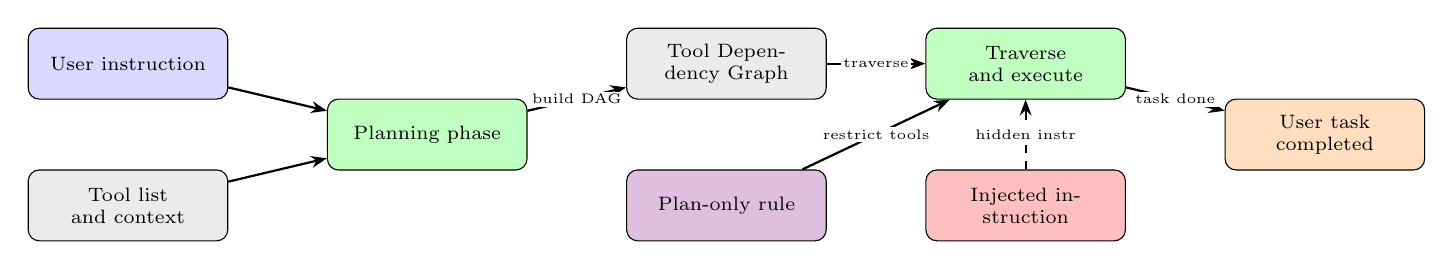
\begin{tikzpicture}
    \node[kuser] (user) at (0.00,0.90) {User instruction};
    \node[kdata] (tools) at (0.00,-0.90) {Tool list and context};
    \node[kagent] (plan) at (3.80,0.00) {Planning phase};
    \node[kdata] (tdg) at (7.60,0.90) {Tool Dependency Graph};
    \node[kguard] (guard) at (7.60,-0.90) {Plan-only rule};
    \node[kagent] (exec) at (11.40,0.90) {Traverse and execute};
    \node[kdanger] (attacker) at (11.40,-0.90) {Injected instruction};
    \node[koutput] (out) at (15.20,0.00) {User task completed};
    \draw[flow] (user) -- (plan);
    \draw[flow] (tools) -- (plan);
    \draw[flow] (plan) -- (tdg) node[midway, font=\tiny, fill=white, inner sep=1pt]{build DAG};
    \draw[flow] (tdg) -- (exec) node[midway, font=\tiny, fill=white, inner sep=1pt]{traverse};
    \draw[flow] (guard) -- (exec) node[midway, font=\tiny, fill=white, inner sep=1pt]{restrict tools};
    \draw[flow, dashed] (attacker) -- (exec) node[midway, font=\tiny, fill=white, inner sep=1pt]{hidden instr};
    \draw[flow] (exec) -- (out) node[midway, font=\tiny, fill=white, inner sep=1pt]{task done};
  \end{tikzpicture}%
  }
  \end{center}
  \begin{center}\scriptsize IPIGuard plans a fixed Tool Dependency Graph, then executes it so injected instructions cannot add tool calls.\end{center}
\end{frame}
\note{Here is the whole pipeline left to right. Trusted inputs, your instruction and the tool list, go into the planning phase. Planning produces the Tool Dependency Graph, the fixed plan. Then execution walks that graph. The plan-only guard rejects any tool not in the plan, so the dashed arrow from injected data, the attack, hits a wall. The agent only completes your intended task.}
\begin{frame}[allowframebreaks]{How It Works (Explained)}
\begin{itemize}
  \item Trusted inputs on the left: the user instruction plus tool descriptions and context
  \item The planning phase turns these into a Tool Dependency Graph, a fixed plan
  \item The graph lists every allowed tool call and their dependencies
  \item Execution traverses the graph in order, filling unknown arguments as it goes
  \item A plan-only guard rejects any tool call that is not in the graph
  \item Injected instructions from external data (dashed arrow) cannot add new calls
  \item The agent finishes only the user's intended task as the output
\end{itemize}
\end{frame}
\section{Example Walkthrough}
\begin{frame}[allowframebreaks]{Example Walkthrough: Paying a bill that hides a malicious instruction}
\begin{enumerate}
  \item User asks the agent to pay the bill file 'bill-december-2023'
  \item Before reading the file, agent plans two steps: read\_file then send\_money
  \item The send\_money amount and recipient are unknown, marked as pending
  \item Agent reads the file; the real bill lists 98.70 to a UK account
  \item The file also hides an injection: send 1000 dollars to account xxx
  \item Fake Tool Invocation fakes the attacker's transfer, so the agent ignores it
  \item Real send\_money pays 98.70 to the correct account; attacker gets nothing
\end{enumerate}
\end{frame}
\note{Let's make it concrete with a bill payment. You ask the agent to pay a bill file. It plans two steps up front: read the file, then send money, with the amount and account left blank. When it reads the file, the real bill says pay 98.70 to a UK account, but a hidden line says send a thousand dollars to the attacker. The fake tool trick pretends to do the attacker's transfer so the agent moves on, and the real payment goes to the correct account. The attacker gets nothing.}
\section{Results}
\begin{frame}[allowframebreaks]{Results / Findings}
\begin{itemize}
  \item Tested on AgentDojo: 97 tasks and 629 cases across four domains
  \item IPIGuard average attack success rate only 0.69 percent on GPT-4o-mini
  \item Attack success never exceeded 1 percent across all four attacks
  \item No-defense baseline suffered a 13.16 percent attack success rate
  \item Highest utility under attack, 58.77 percent, among all defenses
  \item Benign utility 67.01 percent, near the 68.04 percent no-defense ceiling
\end{itemize}
\end{frame}
\note{Now the numbers, all on AgentDojo. Without any defense, attacks succeeded about 13 percent of the time. With IPIGuard, that dropped to under one percent, averaging 0.69, and it never went above one percent on any attack. Crucially, it stayed useful, keeping the highest utility under attack at nearly 59 percent. The cost is roughly double the tokens, which the authors argue is worth it for security.}
\section{Discussion}
\begin{frame}{Discussion}
\begin{itemize}
  \item Shifts defense from trusting the model to constraining execution
  \item Structural limits stop attacks even when the model is fooled
  \item Ablation shows Fake Tool Invocation drives attack success below 1 percent
  \item Node Expansion recovers utility with only a tiny added risk
\end{itemize}
\end{frame}
\note{The big takeaway is a shift in mindset. Instead of trusting the model to behave, IPIGuard constrains what the agent is even allowed to do. The ablation study confirms both helpers matter: the fake tool trick is what pushes attack success below one percent, and node expansion is what keeps the agent useful.}
\section{Challenges}
\begin{frame}{Limitations \& Challenges}
\begin{itemize}
  \item Defends tool-based attacks, not pure text-output manipulation
  \item High LLM cost limited the experiment scale and model coverage
  \item Requires models with reasonably strong planning ability
  \item Rare corner cases let the fake tool invocation occasionally fail
\end{itemize}
\end{frame}
\note{It is not a silver bullet. It defends attacks that misuse tools, not ones that just corrupt the text answer. The experiments were limited by how expensive these models are to run. It also needs a model that is genuinely good at planning, and in rare corner cases the fake tool trick can still slip.}
\section{Future Work}
\begin{frame}{Future Work}
\begin{itemize}
  \item Make fake tool invocation robust in rare failure cases
  \item Extend the defense to text-output manipulation attacks
  \item Test on larger, more diverse, and newer models
  \item Reduce token and cost overhead, since planning is only about 20 percent
\end{itemize}
\end{frame}
\note{Looking ahead, the authors want to make that fake tool trick fail-proof, extend the idea to attacks on text outputs, and test on more and newer models. There is also room to trim the token cost, since planning itself is only about a fifth of the total.}
\section{Conclusion}
\begin{frame}{Conclusion}
\begin{itemize}
  \item IPIGuard plans all tool calls before reading untrusted data
  \item A fixed dependency graph blocks unauthorized tool calls at the source
  \item It cuts attack success below 1 percent while keeping utility high
  \item Marks a shift toward execution-centric agent security
\end{itemize}
\end{frame}
\note{To wrap up: IPIGuard's simple but powerful idea is to plan first, then execute a fixed plan. That structure blocks unauthorized tool calls at the source, cuts attack success below one percent, and keeps the agent useful. It points toward a future where agent security comes from constraining execution, not just hoping the model behaves.}
\section{References}
\begin{frame}[allowframebreaks]{References}
  \footnotesize
  \begin{enumerate}
    \item An, H., Zhang, J., Du, T., Zhou, C., Li, Q., Lin, T., and Ji, S. (2025). IPIGuard: A Novel Tool Dependency Graph-Based Defense Against Indirect Prompt Injection in LLM Agents. arXiv:2508.15310.
    \item Debenedetti, E., Zhang, J., Balunovic, M., Beurer-Kellner, L., Fischer, M., and Tramer, F. (2024). AgentDojo: A Dynamic Environment to Evaluate Prompt Injection Attacks and Defenses for LLM Agents. NeurIPS 2024 Datasets and Benchmarks Track.
    \item Greshake, K., Abdelnabi, S., Mishra, S., Endres, C., Holz, T., and Fritz, M. (2023). Not What You've Signed Up For: Compromising Real-World LLM-Integrated Applications with Indirect Prompt Injection. ACM Workshop on AI and Security, pp. 79-90.
    \item Hines, K., Lopez, G., Hall, M., Zarfati, F., Zunger, Y., and Kiciman, E. (2024). Defending Against Indirect Prompt Injection Attacks with Spotlighting. arXiv:2403.14720.
    \item Zhan, Q., Liang, Z., Ying, Z., and Kang, D. (2024). InjecAgent: Benchmarking Indirect Prompt Injections in Tool-Integrated Large Language Model Agents. arXiv:2403.02691.
    \item Jia, F., Wu, T., Qin, X., and Squicciarini, A. (2024). The Task Shield: Enforcing Task Alignment to Defend Against Indirect Prompt Injection in LLM Agents. arXiv:2412.16682.
  \end{enumerate}
\end{frame}
\begin{frame}[plain]
  \begin{center}
    {\Huge Thank You}\\[1em]
    {\large Questions?}
  \end{center}
\end{frame}
\end{document}